% The role model: the ADK sits one abstraction layer above every PDK and
% reaches each one only through an adapter.
%
% Shared by docs/intro/01_what_is_the_adk.rst and docs/adk/01_architecture.rst.
% Both pages carried the same monospace block; this is the single drawing.
\documentclass[border=3mm]{standalone}
\usepackage{tikz}
\usetikzlibrary{arrows.meta, positioning, calc}
\usepackage[T1]{fontenc}
\usepackage{lmodern}

% IHP colours, matching the other figures in this directory.
\definecolor{IHPfg}{RGB}{0,80,139}
\definecolor{IHPaccent}{RGB}{109,112,114}
\definecolor{IHPlight}{RGB}{225,238,250}

\begin{document}
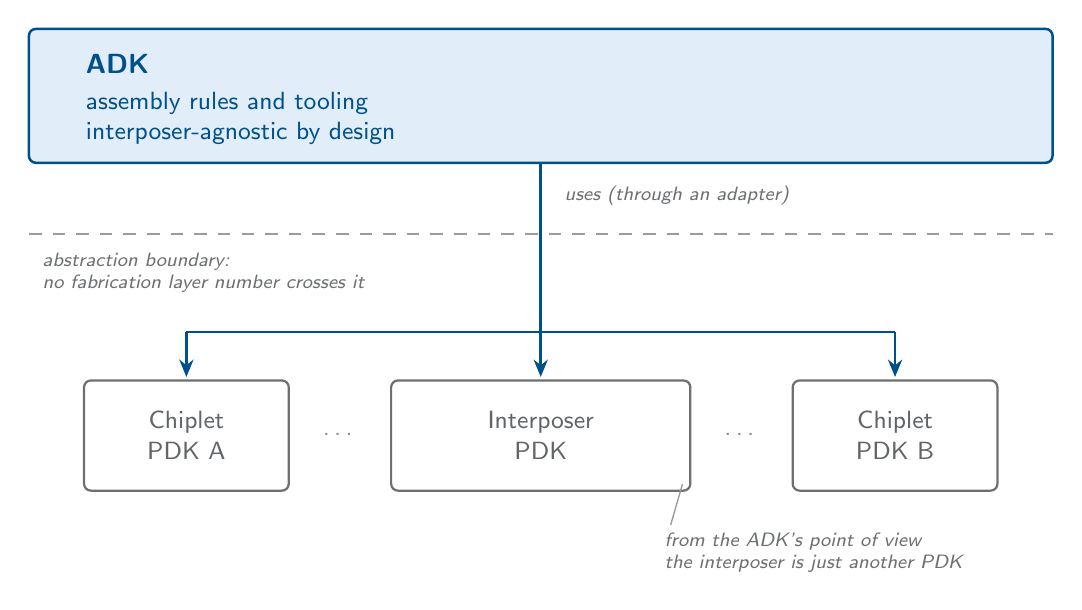
\begin{tikzpicture}[
    >=Stealth,
    % Style names are prefixed adk* so none of them can shadow a tikz key.
    adkroot/.style={
        rectangle, rounded corners=2.5pt,
        draw=IHPfg, fill=IHPlight, line width=0.9pt,
        minimum width=130mm, minimum height=17mm
    },
    adkpdk/.style={
        rectangle, rounded corners=2.5pt,
        draw=IHPaccent, fill=white, line width=0.8pt,
        minimum height=14mm,
        font=\sffamily\small, text=IHPaccent!90!black, align=center
    },
    adkhead/.style={
        font=\sffamily\normalsize\bfseries, text=IHPfg, anchor=west
    },
    adkline/.style={
        font=\sffamily\small, text=IHPfg, anchor=west
    },
    adkstem/.style={
        draw=IHPfg, line width=0.9pt
    },
    adkarrow/.style={
        draw=IHPfg, line width=0.9pt, -{Stealth[length=2.2mm, width=1.8mm]}
    },
    adkbound/.style={
        draw=IHPaccent!70, line width=0.7pt, dash pattern=on 1.6mm off 1.4mm
    },
    adklead/.style={
        draw=IHPaccent!70, line width=0.5pt
    },
    adknote/.style={
        font=\sffamily\scriptsize\itshape, text=IHPaccent, align=left
    },
    adkdots/.style={
        font=\sffamily\small, text=IHPaccent!80
    }
]

% ---- Tier 1: the ADK, one wide box spanning the whole figure ----
\node[adkroot] (adk) at (6.5, -0.85) {};

\node[adkhead] at (0.60, -0.44) {ADK};
\node[adkline] at (0.60, -0.94) {assembly rules and tooling};
\node[adkline] at (0.60, -1.32) {interposer-agnostic by design};

% ---- The abstraction boundary ----
\draw[adkbound] (0, -2.60) -- (13, -2.60);
\node[adknote, anchor=north west] at (0.05, -2.72)
    {abstraction boundary:\\no fabrication layer number crosses it};

% ---- Stem, bus and the three identical descending arrows ----
\draw[adkstem] (6.5, -1.70) -- (6.5, -3.85);
\draw[adkstem] (2.0, -3.85) -- (11.0, -3.85);

\node[adknote, anchor=west] at (6.68, -2.12) {uses (through an adapter)};

\draw[adkarrow] (2.0,  -3.85) -- (2.0,  -4.42);
\draw[adkarrow] (6.5,  -3.85) -- (6.5,  -4.42);
\draw[adkarrow] (11.0, -3.85) -- (11.0, -4.42);

% ---- Tier 2: the PDKs, all reached the same way ----
\node[adkpdk, minimum width=26mm, anchor=north] (pdka) at (2.0,  -4.45)
    {Chiplet\\PDK A};
\node[adkpdk, minimum width=38mm, anchor=north] (pdki) at (6.5,  -4.45)
    {Interposer\\PDK};
\node[adkpdk, minimum width=26mm, anchor=north] (pdkb) at (11.0, -4.45)
    {Chiplet\\PDK B};

% The set is open.
\node[adkdots] at (3.95, -5.15) {\ldots};
\node[adkdots] at (9.05, -5.15) {\ldots};

% ---- The point the diagram exists to make ----
\draw[adklead] (8.30, -5.78) -- (8.15, -6.30);
\node[adknote, anchor=north west] at (7.95, -6.28)
    {from the ADK's point of view\\the interposer is just another PDK};

\end{tikzpicture}
\end{document}
